% opis interfejsu graficznego aplikacji

\section{Interfejs graficzny}
Wygląd interfejsu graficznego aplikacji przedstawiony jest na rysunku \ref{fig:gui}.

\begin{figure}
 \begin{center} 
  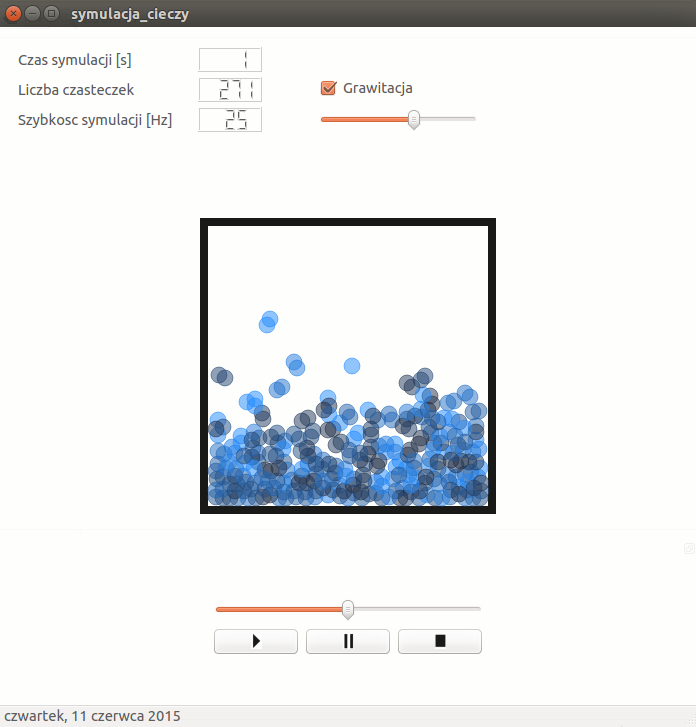
\includegraphics[width=\textwidth]{./rysunki/gui} 
 \end{center}
 \caption{Interfejs graficzny aplikacji}
 \label{fig:gui} 
\end{figure}

W centralnej części aplikacji widoczny jest jej główny element, czyli zbiornik z~cząsteczkami. Pod nim znajduje się \textit{slider} pozwalający na przechylanie zbiornika.

Cząsteczki oraz okienko aplikacji są częściowo przezroczyste, co pozwala na obserwowanie elementów znajdujących za cieczą.

Użytkownik za pomocą trzech przycisków umiejscowionych na dole ekranu może sterować symulacją, a mianowicie ją: uruchomić, zamrozić lub zatrzymać.  

W lewej górnej części okienka znajdują się elementy informacyjne pozwalające śledzić parametry symulacji: jej czas trwania, symulowaną liczbę cząsteczek oraz szybkość odświeżania wizualizacji. Na prawo od nich umiejscowione są elementy umożliwiające interakcję użytkownika z aplikacją: \textit{slider} pozwalający na zmianę szybkości symulacji oraz pole typu \textit{checkbox} zmieniające wektor grawitacji.

Na widocznej w dole ekranu belce statusowej wyświetlana jest aktualna data. W~pasku menu dostępna jest opcja zamknięcia aplikacji.

Rozkład elementów interfejsu graficznego jest odpowiednio modyfikowany przy zmianie wymiarów okienka.